%************************************************
\chapter{Value Iteration with CVaR}\label{ch:vi}
%************************************************

Value iteration is a standard algorithm for maximizing expected discounted reward used in reinforcement learning. In this chapter we extend the results of \citet{chow2015risk}, who have recently proposed an approximate value iteration algorithm for CVaR MDPs. 

The original algorithm requires the computation of a linear program in each step of the value iteration procedure. Utilizing a connection between the used $\alpha \cvar_\alpha$ function and the quantile function, we sidestep the need for this computation and propose a linear-time version of the algorithm, making CVaR value iteration feasible for much larger MDPs. 

We first present the original algorithm in section \ref{sec:vi:cvar}. The improved algorithm is presented in section \ref{sec:vi:linear}. In section \ref{sec:vi-experiments}, we test the algorithm on selected environments.

%*****************************************

\section{CVaR Value Iteration}\label{sec:vi:cvar}

\citet{chow2015risk} present a dynamic programming formulation for the CVaR MDP problem (see section \ref{sec:prelim:problem}). \todo{more} We repeat their key ideas and results bellow, as they form a basis for our contributions presented in later sections. The results are presented with our notation introduced in chapter \ref{ch:prelim}, which differs slightly from the paper, but the core ideas remain the same.

\subsection{Bellman Equation for CVaR}

The results of \citet{chow2015risk} heavily rely on the CVaR decomposition theorem \cite{decomp}:

\unclear{repeat the original theorems in full?}

\begin{equation}\label{eq:vi:cvardecomp}
CVaR_\alpha\bround{Z^\pi(x, a)} = \min_{\xi \in \envelope} \sum_{x'} p(x'| x, a)\xi(x') CVaR_{\xi(x')\alpha}\bround{Z^\pi(x')}
\end{equation}

where the risk envelope $\envelope$ coincides with the dual definition of CVaR \ref{eq:prelim:envelope}.

The theorem states that we can compute the $CVaR_\alpha\bround{Z^\pi(x, a)}$ as the minimal (or worst-case) weighted combination of $CVaR_\alpha\bround{Z^\pi(x')}$ under a probability distribution perturbed by $\xi(x')$.

Note that the decomposition requires only the representation of CVaR at different (or all) confidence levels and no the whole distribution. \todo{make the distinction clear, maybe in prelim?}.

\citet{chow2015risk} extend these results by defining the \emph{CVaR value-function} $V(x, y)$ with an augmented state-space $\mathcal{X}\times\mathcal{Y}$ where $\mathcal{Y}=(0,1]$ is an additional continuous state.

\begin{equation}
V(x, y)=\max_{\pi \in \Pi} \cvar_{y}\bround{Z^\pi(x)}
\end{equation}

Similar to standard DP, it is convenient to work with with operators defined on the space of value functions. This leads to the following definition of the CVaR Bellman operator $\mathbf{T}:\mathcal{X}\times\mathcal{Y}\to\mathcal{X}\times\mathcal{Y}$:

\begin{equation}
\mathbf{T}V(x, y) = \max_a \bsquare{ R(x, a) + \gamma \min_{\xi \in \envelope} \sum_{x'} p(x'| x, a)\xi(x') V\bround{x', y\xi(x')}}
\end{equation}

or in our simplified notation:
\begin{equation}\label{eq:vi:tcvar}
\mathbf{T} CVaR_y(Z(x))=\max_a \bsquare{R(x, a) + \gamma CVaR_{y}(Z(x, a))}
\end{equation}

\citep{chow2015risk}(lemma 3) showed that the operator $\mathbf{T}$ is a contraction and also perserves the convexity of $y CVaR_t$. The maximization problem \ref{eq:vi:cvardecomp} is a convex one and therefore has a unique solution. Additionally, the fixed point of this contraction is the optimal $V^*(x, y) = \max_{\pi \in \Pi} CVaR_y (Z^\pi(x, y))$ (Theorem 4).
 
The value-function $V^*$ can then be used to extract the optimal policy $\pi^*$ of the original problem \ref{eq:prelim:problem}, using the following theorem

\begin{theorem}[Optimal Policies, Theorem 5 in \citep{chow2015risk}]\label{thm:vi:optimalpolicy}
Let $\pi_H^*=\{\mu_0,\mu_1,\ldots\}\in\Pi_H$ be a history-dependent policy recursively defined as:
\begin{equation}\label{eq:policy_construct}
\mu_k(h_k) = u^*(x_k, y_k),\,\,\forall k\geq 0,
\end{equation}
with initial conditions $x_0$ and $y_0=\alpha$, and state transitions
\begin{equation}\label{eq:opt_state}
x_k\sim P(\cdot\mid x_{k-1},u^*(x_{k-1},y_{k-1})),\quad y_k = y_{k-1}\xi_{x_{k-1},y_{k-1},u^*}^*(x_k), \forall k\geq 1,
\end{equation}
where the stationary Markovian policy $u^*(x,y)$ and risk factor $\xi_{x,y,u^*}^*(\cdot)$ are solution to the  min-max optimization problem in the CVaR Bellman operator $\mathbf T[V^*](x,y)$.
Then, $\pi^*_H$ is an optimal policy for problem \eqref{eq:prelim:problem} with initial state $x_0$ and CVaR confidence level $\alpha$.
\end{theorem}


This algorithm is unfortunately unusable in practice, as the state-space is continuous in $y$. The solution proposed in \cite{chow2015risk} is then to represent the convex $y CVaR_y$ as a piecwise linear function. 

\subsection{Value Iteration with Linear Interpolation}

Given a set of $N(x)$ interpolation points $\mathbf{Y}(x) = \braces{y_1, \dots, y_{N(x)}}$, we can interpolate the $yV(x,y)$ function on these points, i.e.

\begin{equation*}
\interpI_{x}[V](y)=y_iV(x,y_{i})+\frac{y_{i+1}V(x,y_{i+1})-y_iV(x,y_{i})}{y_{i+1}-y_i}(y-y_i),
\end{equation*}

where $y_i = \max \left\{y'\in \mathbf{Y}(x) : y' \leq y\right\}$
The interpolated Bellman operator is then also a contraction and has a bounded error(Theorem 7). 

\todo{bounded -> linear in $\theta$}

\begin{equation}\label{eq:vi:linearbellman}
\mathbf{T}_\interpI V(x, y) = \max_a \bsquare{ R(x, a) + \gamma \min_{\xi \in \envelope} \sum_{x'} p(x'| x, a)\dfrac{\interpI_{x'} [V](y\xi(x'))}{y}}
\end{equation}

The full value iteration procedure is presented in algorithm \ref{alg:vi:cvarlinear}

\begin{algorithm}[h]
\caption{\texttt{CVaR Value Iteration with Linear Interpolation}}\label{alg:vi:cvarlinear}
1: \textbf{Given:}
\begin{itemize}
%\item An interpolation error bound $\epsilon>0$ for small CVaR thresholds.
\item $N(x)$ interpolation points $\mathbf{Y}(x)  = \left\{y_1,\dots,y_{N(x)}\right\} \in [0,1]^{N(x)}$ for every $x\in \mathcal X$ with $y_i<y_{i+1}$, $y_1=0$ and $y_{N(x)}=1$.
%, $y_2 = \min_{x',a}\{ P(x'|x,a):P(x'|x,a)\neq 0\}$
%\item An interpolation function $\interpI_{x}[V](y;\interpY(x))$ for $yV(x,y)$ for any arbitrary value function $V$.
\item Initial value function $V_0(x,y)$ that satisfies Assumption \ref{ass:V_0}.
 %where $V_0(x,y)=0$ at $y<0$.
\end{itemize}
2: For $t = 1,2,\dots$
\begin{itemize}
%\item Update the smallest non-zero grid $y_2$ in $\interpY(x)$ by choosing it to satisfy $\max_{x\in\mathcal X, y\in \mathbf I_2(x)}|V_0(x,y_2)-V_0(x,y)|\leq\epsilon$, where the interpolation based Bellman operator $ \bellint$ is given by
%  \[
%\hspace{-0.5in}  \bellint[V](x,y) =
% \min_{a\in\mathcal A}\left[C(x,a)+\gamma\max_{\xi\in \U_{\text{CVaR}}(y, P(\cdot|x,a))}\sum_{x'\in\mathcal X}\frac{\interpI_{x'}[V](y\xi(x');\interpY(x'))}{y}P(x'|x,a)\right].
%   \]
\item For each $x \in \mathcal X$ and each $y_i\in \mathbf{Y}(x)$, update the value function estimate as follows:
  \begin{equation*}
   V_t(x,y_i)= \mathbf{T}_\interpI[V_{t-1}](x,y_i),
  \end{equation*}
  \end{itemize}
3: Set the converged value iteration estimate as $\widehat{V}^*(x,y_i)$, for any $x\in\mathcal X$, and $ y_i\in\mathbf{Y}(x)$.
\end{algorithm}

This algorithm can be used to find an approximate global optimum in any MDP. There is however the issue of computational complexity. As the algorithm stands, the straightforward approach is to solve each iteration of \ref{eq:vi:linearbellman} as a linear program, since the problem is convex and piecewise linear. This however is not practical, as the LP computation can be demanding and is therefore not suitable for large state-spaces.

\unclear{maybe formulate the LP exactly?}

In the next section we aim to find a different way of computing the optimization problem presented in \ref{eq:vi:cvardecomp}.


%*****************************************

\section{Efficient computation using quantile representation}\label{sec:vi:linear}

We note several important facts regarding the CVaR computation. Firstly, it is unimportant \emph{how} we arrive at the $\cvar_y(Z(x, a))$ present in the CVaR Bellman operator \ref{eq:vi:tcvar}. Secondly, note that any discrete distribution has a piecewise linear $y\cvar_y$ function \cite{rockafellar2002conditional}, and this statement is twosided: any a piecewise linear $y\cvar_y$ function can be seen as representing a certain discrete distribution.

The relation between $y\cvar_y$ and the underlying distribution is best described in the following equation:

\begin{equation}\label{eq:vi:varcvarderivation}
\dfrac{\partial}{\partial \alpha} \alpha \cvar_\alpha(Z) = \dfrac{\partial}{\partial \alpha} \int_0^\alpha VaR_\beta(Z) d\beta = VaR_\alpha(Z)
\end{equation}

We see that the quantile function of $Z$ is extractable from the $y\cvar_y$ function by differentiating over $y$ \todo{unify $y, \alpha$}. The opposite direction also holds:

\begin{equation}\label{eq:vi:varcvarintegration}
\alpha \cvar_\alpha(Z) = \int_0^\alpha VaR_\beta(Z) \dt \beta + c
\end{equation}

where we have $c=0$ because of a starting condition $y \cvar_y \given[\Big]_{y=0}=0$.

\subsection{CVaR Computation via Quantile Representation}

We propose the following procedure: instead of using linear programming for the CVaR computation, we use the underlying distributions represented by the $\alpha CVaR_\alpha$ function to compute CVaR.

The computation of CVaR of a discrete probability mixture is a linear-time process as we show bellow. The general steps of the computation are as follows

\begin{enumerate}
\item transform $y \cvar_y$ of each possible state transition to a discrete probability distribution function using \ref{eq:vi:varcvarderivation}
\item combine these to to a distribution representing the full state-action distribution
\item compute $y \cvar_y$ for all atoms using \ref{eq:vi:varcvarintegration}
\end{enumerate}

\begin{figure}[h]
\center
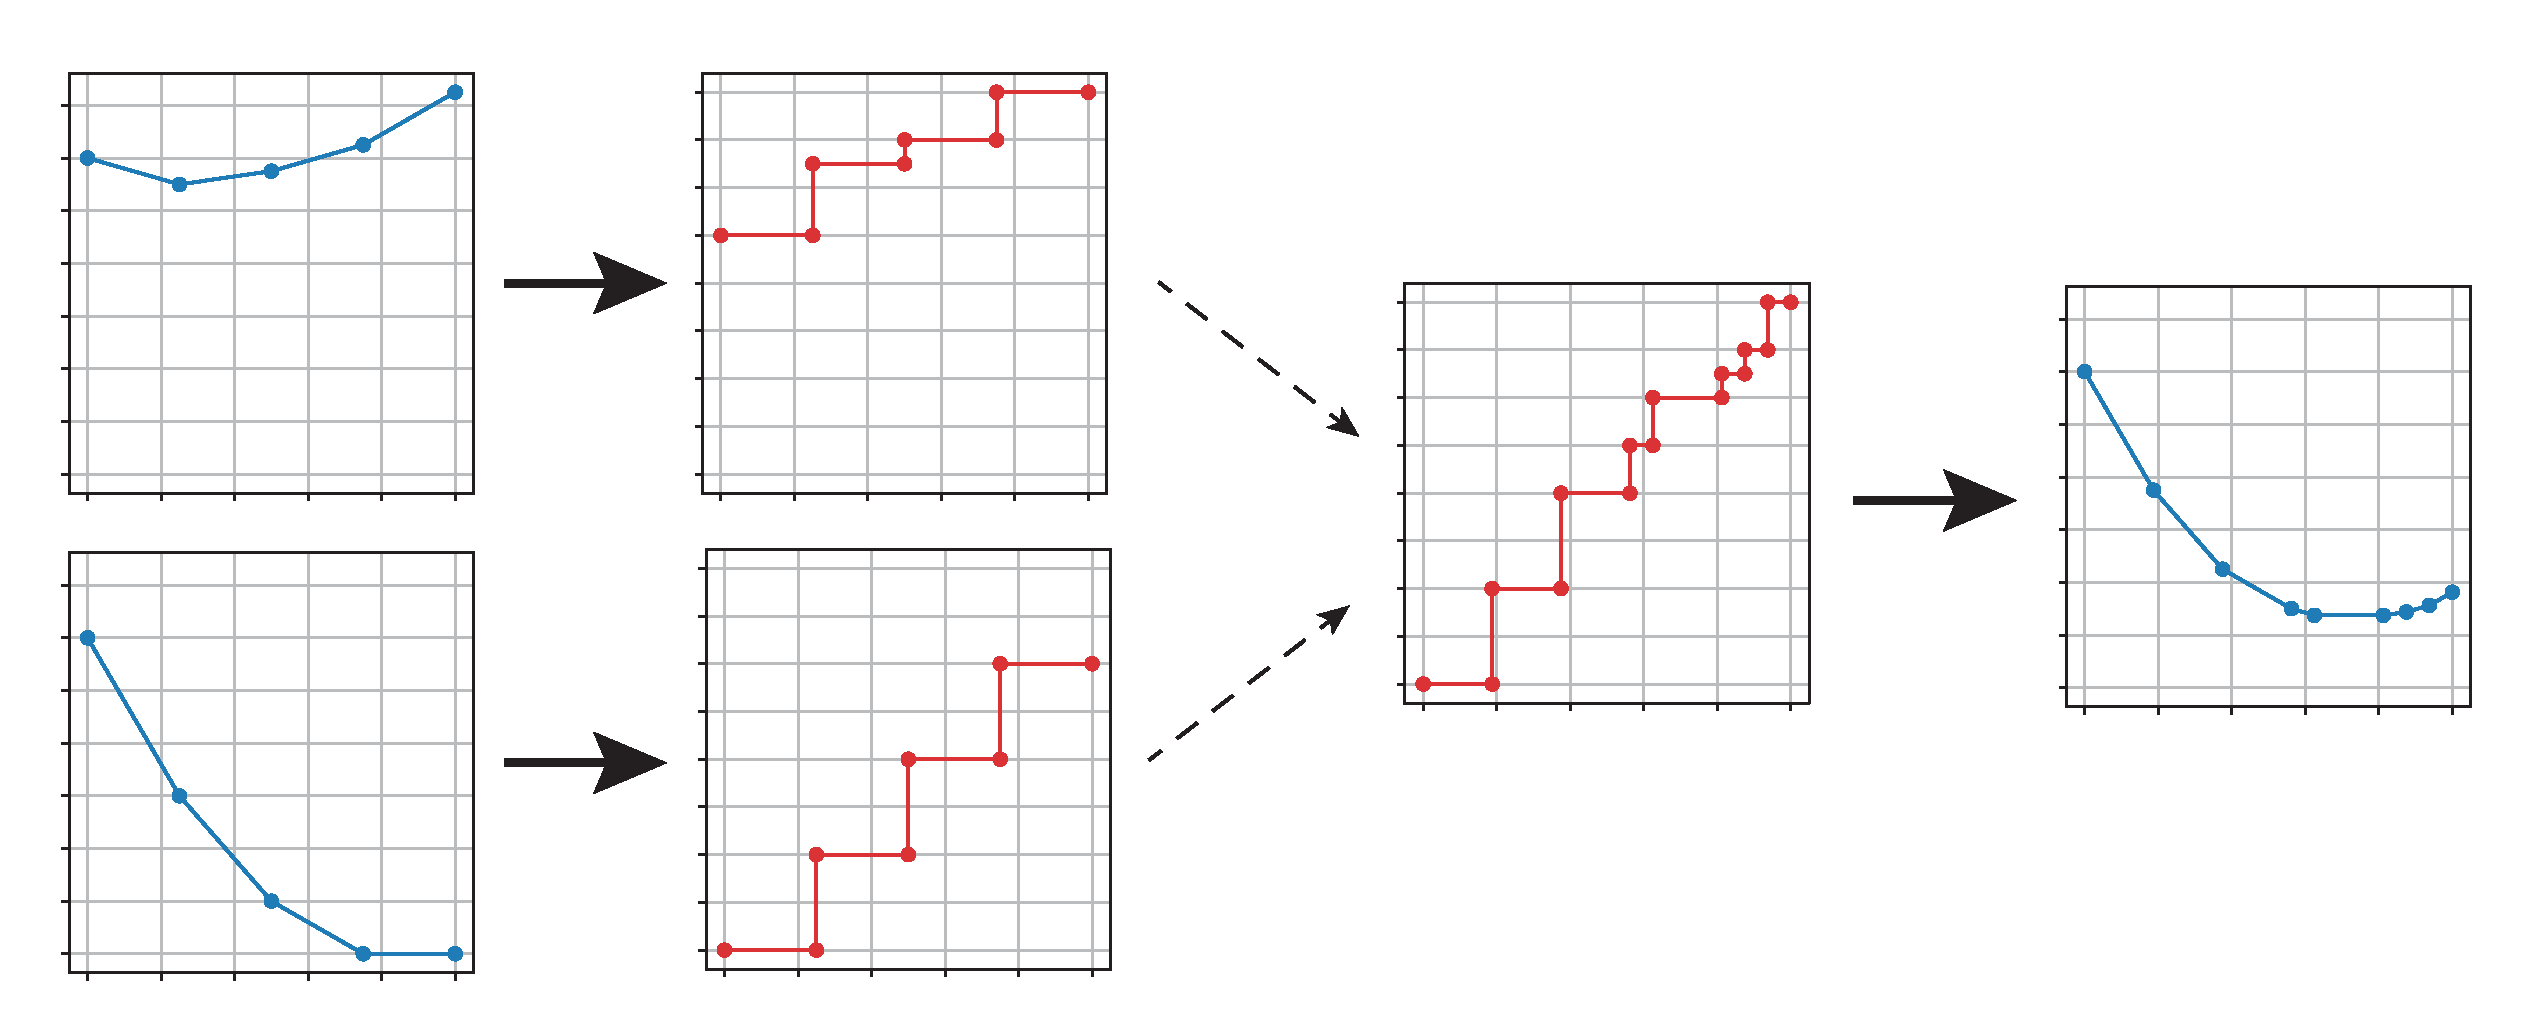
\includegraphics[width=\linewidth]{gfx/cvar_vi_conversion.pdf}
\caption{Visualization of the CVaR Value Iteration for a single state and action with two transition states. Thick arrows represent the conversion between $\acvara$ and the quantile function.}
\end{figure}

%\begin{algorithm}
%\caption{CVaR computation}
%
%\begin{multicols}{2}
%
%\begin{algorithmic}
%    \STATE \textbf{input} $\alpha, x_t, \pi_\text{old}, \gamma$
%    \WHILE{$x_t$ is not terminal}
%    	\STATE $a = \text{arg}\max_a CVaR_\alpha(Z(x_t, a))$
%		\STATE $s = VaR_\alpha(Z(x_t, a))$
%		\columnbreak
%
%    	\STATE $x_t, r_t = \text{envTransition}(x_t, a)$
%    	\STATE $\alpha = F_{Z(x_t, \pi_\text{old}(x_t))}\left(\dfrac{s - r}{\gamma}\right) $ \textcolor{gray}{\# $VaR_\alpha(Z(x_t, \pi_\text{old}(x_t))) == \dfrac{s - r}{\gamma}$}
%   	\ENDWHILE
%\end{algorithmic}
%\end{multicols}
%\end{algorithm}
%
%\begin{minipage}[t]{0.5\linewidth}
%  \vspace{0pt}  
%  \begin{algorithm}[H]
%    \caption{Algo 1}
%    line 1\;
%    line 2\;
%  \end{algorithm}
%\end{minipage}%
%\begin{minipage}[t]{5cm}
%  \vspace{0pt}
%  \begin{algorithm}[H]
%    \caption{Algo 1}
%    line 1\;
%  \end{algorithm}
%\end{minipage}

\unclear{proof necessary? also, maybe it is already in the $\xi$ proof}

\subsection{$\xi$-computation}

Similarly to theorem \ref{thm:vi:optimalpolicy}, we need a way to compute the $y_{k+1}=y_{k}\xi^*(x_k)$ to extract the optimal policy. Again, we can skip the LP computation by using the following intuition: $y_{k+1}$ is the portion of $Z(x_{k+1})$ that is present in $\cvar_{y_k}(Z(x_k))$. In the continuous case, it is the probability in $Z(x_{k+1})$ before the $\var_{y_k}(Z(x_k))$ as we show bellow.

\todo{proof for discrete distributions}

\begin{theorem}
Solution to minimization problem \ref{eq:vi:cvardecomp} can be computed without optimization by setting
\begin{equation}\label{eq:xi-claim}
\xi ( x' ) = \dfrac{F_{x'}(F^{-1}_x(\alpha))}{\alpha} 
\end{equation}
\end{theorem}

\begin{proof}
For simplification, we work only with two states: $x'$ the actual sampled state and $\bar{x}'$ representing the other states. The equation then simplifies to

\begin{equation}\label{eq:cvardecomp2}
\begin{split}
CVaR_\alpha(x, a)&=\min_{\xi} \, p\xi CVaR_{\xi\alpha}(x') + (1-p)\dfrac{1-p\xi}{1-p}CVaR_{\frac{1-p\xi}{1-p}\alpha}(\bar{x}')\\
&=\min_{\xi} \, p\xi CVaR_{\xi\alpha}(x') + (1-p\xi)CVaR_{\frac{1-p\xi}{1-p}\alpha}(\bar{x}')\\
\end{split}
\end{equation}

To find the min we first find the first derivative\footnote{
We used the following identities:
\begin{equation*}
\dfrac{\partial CVaR_{\alpha\xi}}{\partial \xi} = \frac{1}{\xi}VaR_{\xi\alpha}-\frac{1}{\xi}CVaR_{\xi\alpha}\quad\quad\quad
\dfrac{\partial CVaR_{\frac{1-p\xi}{1-p}\alpha}}{\partial\xi} = \frac{p}{1-p\xi}CVaR_{\frac{1-p\xi}{1-p}\alpha}	-	\frac{p}{1-p\xi}VaR_{\frac{1-p\xi}{1-p}\alpha}
\end{equation*}
} w.r.t. $\xi$

\begin{equation}
\begin{split}
\dfrac{\partial CVaR_\alpha}{\partial \xi} &= pCVaR_{\xi\alpha} + p\xi \dfrac{\partial CVaR_{\alpha\xi}}{\partial \xi} - pCVaR_{\frac{1-p\xi}{1-p}\alpha} + (1 - p\xi)\dfrac{\partial CVaR_{\frac{1-p\xi}{1-p}\alpha}}{\partial\xi}\\
&= pCVaR_{\xi\alpha} + p\xi\left[	\frac{1}{\xi}VaR_{\xi\alpha}-\frac{1}{\xi}CVaR_{\xi\alpha}	\right] - pCVaR_{\frac{1-p\xi}{1-p}\alpha} \\&\hspace*{5cm} + (1-p\xi)\left[	\frac{p}{1-p\xi}CVaR_{\frac{1-p\xi}{1-p}\alpha}	-	\frac{p}{1-p\xi}VaR_{\frac{1-p\xi}{1-p}\alpha}\right]\\
&= pCVaR_{\xi\alpha} + pVaR_{\xi\alpha} - pCVaR_{\xi\alpha} - pCVaR_{\xi\alpha} - pCVaR_{\frac{1-p\xi}{1-p}\alpha} \\&\hspace*{5cm} + CVaR_{\frac{1-p\xi}{1-p}\alpha} - pVaR_{\frac{1-p\xi}{1-p}\alpha}\\
&= pVaR_{\xi\alpha} - pVaR_{\frac{1-p\xi}{1-p}\alpha}
\end{split}
\end{equation}

By setting the derivative to 0 (to find the min), we get
\begin{equation}\label{eq:vi:varvar}
VaR_{\xi\alpha}(x')= VaR_{\frac{1-p\xi}{1-p}\alpha}(\bar{x}')
\end{equation}

By inserting claim \ref{eq:xi-claim} into \ref{eq:varvar} we get the symmetrical claim
\begin{equation}
\dfrac{1-p\xi}{1-p} = \xi(\bar{x}') = \dfrac{F_{\bar{x}'}(F^{-1}_x(\alpha))}{\alpha}
\end{equation}

We rewrite \ref{eq:cvardecomp2} as (assuming $\xi$ is the minimum point)

\begin{equation}
\begin{split}
\frac{1}{\alpha} \int_0^\alpha F^{-1}_{x}(t)dt &= p\xi \frac{1}{\xi\alpha} \int_0^{\xi\alpha} F^{-1}_{x'}(t)dt + (1-p\xi)\frac{1-p}{(1-p\xi)\alpha} \int_0^{\frac{1-p\xi}{1-p}\alpha} F^{-1}_{\bar{x}'}(t)\\
&=p \frac{1}{\alpha} \int_0^{\xi\alpha} F^{-1}_{x'}(t)dt + (1-p)\frac{1}{\alpha} \int_0^{\frac{1-p\xi}{1-p}\alpha} F^{-1}_{\bar{x}'}(t)
\end{split}
\end{equation}

This must also hold if we multiply both sides by $\alpha$
\begin{equation}
\int_0^\alpha F^{-1}_{x}(t)dt = p\int_0^{\xi\alpha} F^{-1}_{x'}(t)dt + (1-p)\int_0^{\frac{1-p\xi}{1-p}\alpha} F^{-1}_{\bar{x}'}(t)
\end{equation}
And we take derivations w.r.t. $\alpha$ of both sides
\begin{equation}
F^{-1}_{x}(\alpha) = p\xi F^{-1}_{x'}(\xi\alpha) + (1-p\xi) F^{-1}_{\bar{x}'}(\frac{1-p\xi}{1-p}\alpha)
\end{equation}


By inserting \ref{eq:xi-claim} we get
\begin{equation}
\begin{split}
 p\xi F_{x'}^{-1}(\xi\alpha) + (1-p)\xi_2 F_{\bar{x}'}^{-1}\left(\xi_2\alpha\right) &= p\xi F_{x'}^{-1}(F_{x'}(F^{-1}_x(\alpha))) + (1-p\xi) F_{\bar{x}'}^{-1}\left(F_{\bar{x}'}(F^{-1}_x(\alpha))\right)\\
 &= p\xi F_x^{-1}(\alpha) + (1-p\xi)F_x^{-1}(\alpha) = F_x^{-1}(\alpha)
\end{split}
\end{equation}

We've shown that the proposed solution \ref{eq:xi-claim} satisfies the minimization constraint \ref{eq:vi:varvar} (= is a minimal point) and satisfies the dual decomposition \ref{eq:vi:cvardecomp}. (This has been shown only in the differentiated form )

\end{proof}


%*****************************************



\section{Experiments}\label{sec:vi-experiments}

\todo{$|\mathcal{X}|\sim 1M$ tabular environment}

\todo{get matlab code from tamar}

\subsection{Cliffworld}

\section{Summary}


%*****************************************
%*****************************************
%*****************************************
%*****************************************
%*****************************************



